\documentclass[pdf,contemporain,slideColor,nocolorBG,accumulate,nototal]{prosper}

\title{Genome Center \\
 Cluster}

\begin{document}

\begin{slide}{Genome Center Clusters}
\begin{center}
	
\includegraphics{genbanner.eps}
\end{center}
\end{slide}

%-----------------

\begin{slide}{Introduction}
``If you were plowing a field, which would you rather use: Two strong oxen 
or 1024 chickens?''

--Seymour Cray
\end{slide}

\overlays{6}{%
\begin{slide}{Introduction}
\begin{itemstep}
	\item What is a cluster?
	\begin{itemize}
		\item A collection of machines that work together
	\end{itemize}
	\item Why use a cluster?
	\begin{itemize}
		\item Chickens are cheaper than oxen
		\item {\tiny and easier to feed}
		\item ...but try making 1024 chickens move in the same direction
	\end{itemize}
\end{itemstep}
\end{slide}}

\overlays{6}{%
\begin{slide}{Clusterable Jobs}
\begin{itemstep}
	\item Parallel
	\begin{itemize}
		\item fine-grained parallel
		\item course-grained parallel
		\item embarrassingly parallel
	\end{itemize}
	\item Serial
	\begin{itemize}
		\item Can still benefit from a cluster environment
	\end{itemize}
\end{itemstep}
\end{slide}}

%-----------------

\overlays{3}{%
\begin{slide}{Available Resources}
\begin{itemstep}
	\item genbeo
	\item shiraz
	\item apple
\end{itemstep}
\end{slide}}

%-----------------

\overlays{9}{%
\begin{slide}{Genbeo}
\begin{itemstep}
	\item 19 nodes
	\item Dual Opteron
	\item 4G memory per node
	\item Gigabit ethernet interconnect
	\item 3.2TB storage
	\begin{itemize}
		\item 800G User home dirs and mysql
		\item 800G Shared applications
		\item 800G Shared filesystem
		\item 800G backups
	\end{itemize}
\end{itemstep}
\end{slide}}

%-----------------

\overlays{8}{%
\begin{slide}{Shiraz}
\begin{itemstep}
	\item 110 nodes
	\item Dual processor, dual core Opteron (4 cores/node)
	\item 32 nodes with 8G, remainder with 4G
	\item Gigabit ethernet interconnect
	\item 4.4TB attached storage
	\begin{itemize}
		\item 1.2T User storage
		\item 1.6T shared databases (PDB, blastdb, ...)
		\item 1.6T Shared filesystem
	\end{itemize}
\end{itemstep}
\end{slide}}

\overlays{7}{%
\begin{slide}{Apple}
\begin{itemstep}
	\item 37 nodes
	\item Dual PowerPC G4
	\item 1-2G memory per node
	\item Gigabit ethernet interconnect
	\item 1.6TB attached storage
	\begin{itemize}
		\item 800G User home directories
		\item 800G Mysql and postgres databases
	\end{itemize}
\end{itemstep}
\end{slide}}

\begin{slide}{The Big Picture}
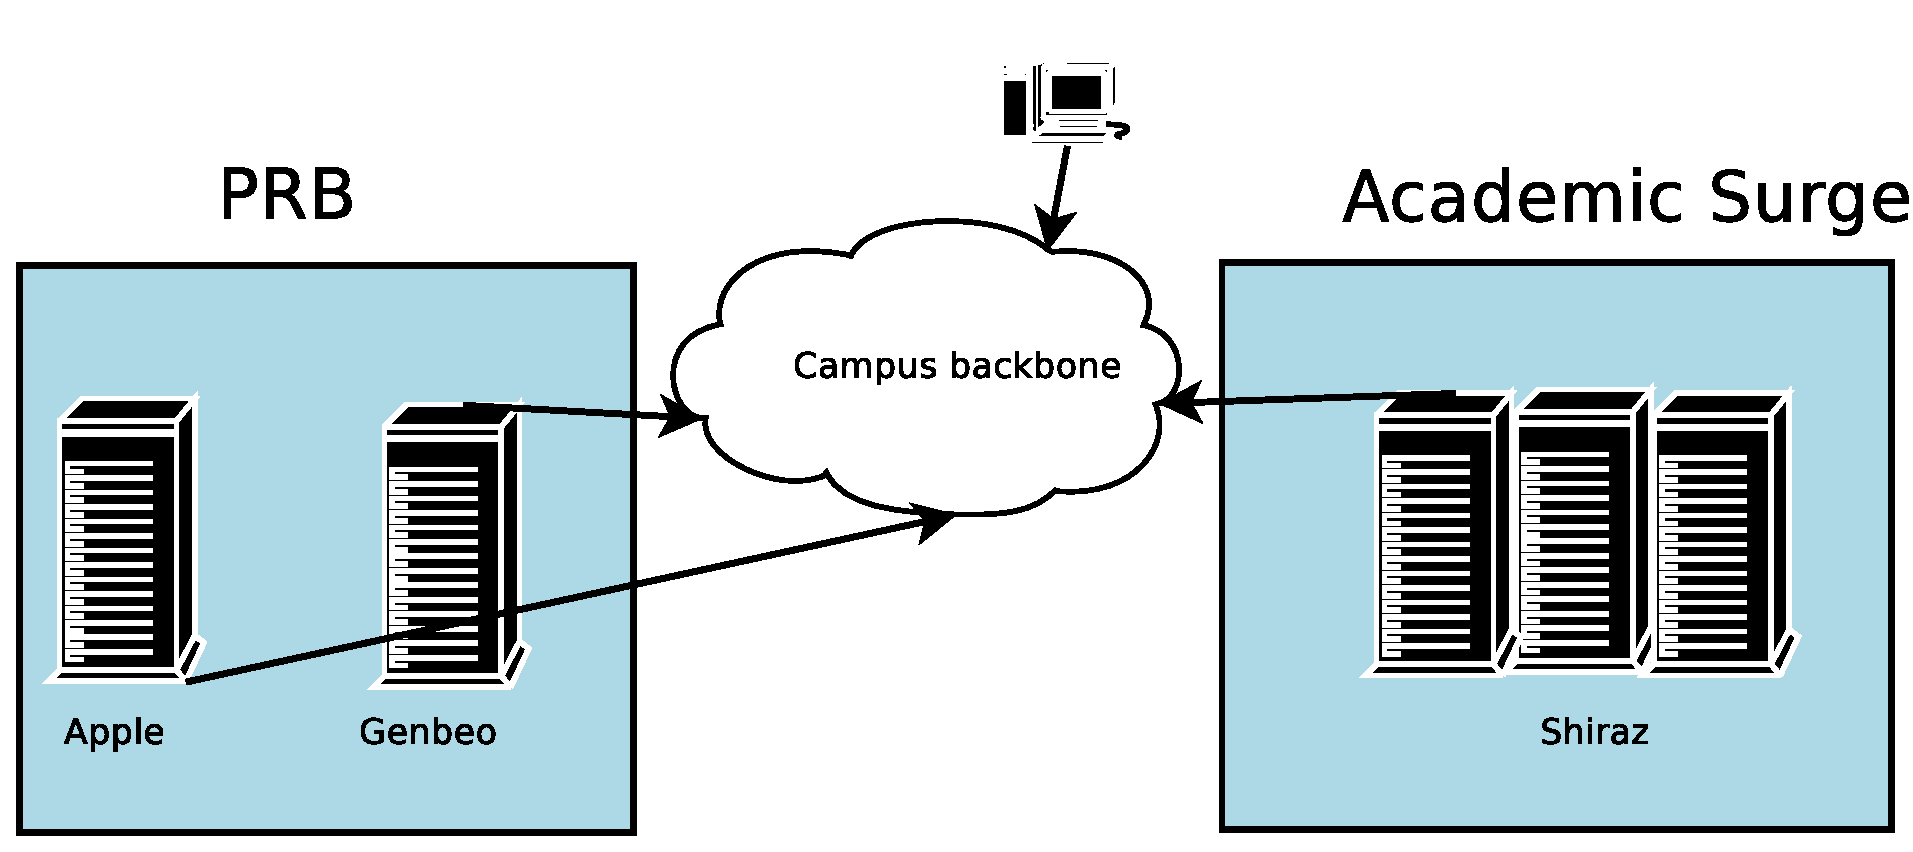
\includegraphics[width=11cm]{network.eps}
\end{slide}

\begin{slide}{Anatomy of a Cluster}
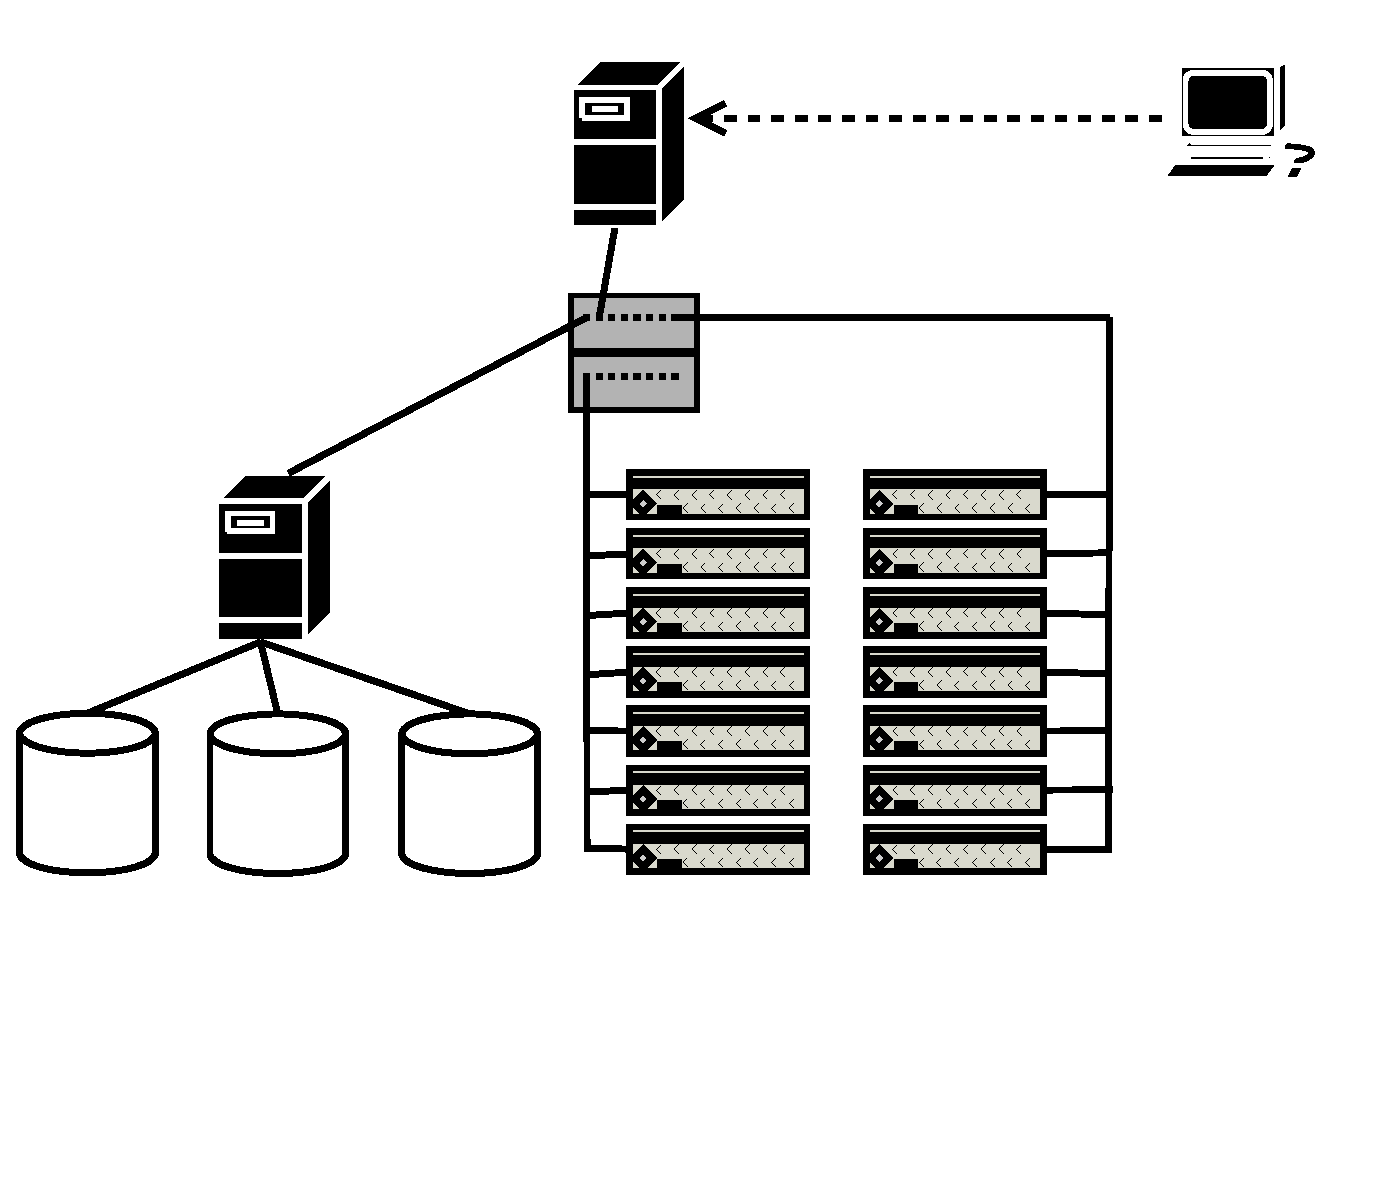
\includegraphics[height=8cm]{cluster_network.eps}
\end{slide}

\overlays{4}{%
\begin{slide}{Available Software}
\begin{itemstep}
	\item Biological databases: 
		\begin{itemize}
			\item pdb
			\item blastdb
			\item ..
		\end{itemize}
\end{itemstep}
\end{slide}}

\overlays{3}{%
\begin{slide}{Available Software}
Compilers
\begin{itemstep}
	\item Gnu compiler suite
	\item Pathscale floating license
	\item Intel?
\end{itemstep}
\end{slide}}

\begin{slide}{Available Software}
\begin{itemize}
	\item biopython
	\item clustalw
	\item EMBOSS
	\item BLAST
	\item HMMER
	\item mrbayes
	\item t-coffee
	\item phylip
	\item ...
\end{itemize}
\end{slide}

\overlays{3}{%
\begin{slide}{Available Software}
\begin{itemstep}
	\item R
	\item mysql
	\item Request your app!
\end{itemstep}
\end{slide}}

\begin{slide}{Your Cluster Account}
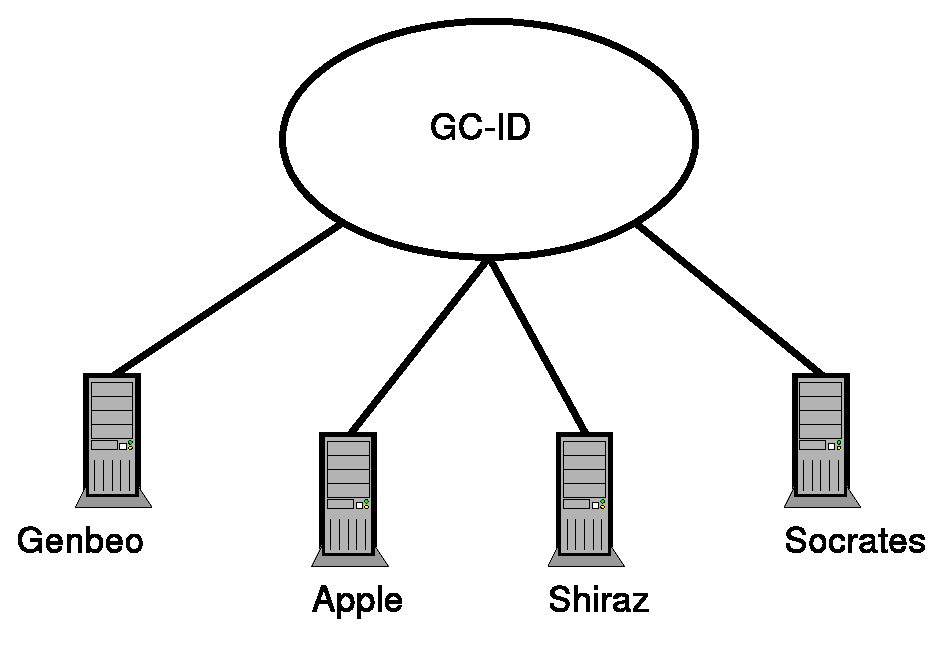
\includegraphics[width=7cm]{central-auth.eps} \\
Same username/password works on all hosts on which you have an account.
\end{slide}

\overlays{3}{%
\begin{slide}{Accessing the cluster}
\begin{itemstep}
	\item Access using ssh
	\item Transfer files using scp/sftp/rsync
	\item Web interface
\end{itemstep}
\end{slide}}

\overlays{7}{%
\begin{slide}{Accessing the cluster: ssh}
\begin{itemstep}
	\item {\tiny \tt ssh username@genbeo.genomecenter.ucdavis.edu}
	\item Add {\tt -X} option (capital!) to forward X connections
	\item Clients for windows:
	\begin{itemize}
		\item putty (free!)
		\item SecureCRT 
		\item ssh.com
		\item winscp
	\end{itemize}
\end{itemstep}
\end{slide}}

\overlays{6}{%
\begin{slide}{Accessing the cluster: copying data}
\begin{itemstep}
	\item scp
	\begin{itemize}
		\item {\tiny \tt scp file username@genbeo:}
	\end{itemize}
	\item rsync
	\begin{itemize}
		\item {\tiny \tt rsync -a directory username@genbeo:}
	\end{itemize}
	\item sftp
	\begin{itemize}
		\item ftp-like interface that works over ssh
	\end{itemize}
\end{itemstep}
\end{slide}}

\begin{slide}{Cluster Web Interface}
\begin{center}
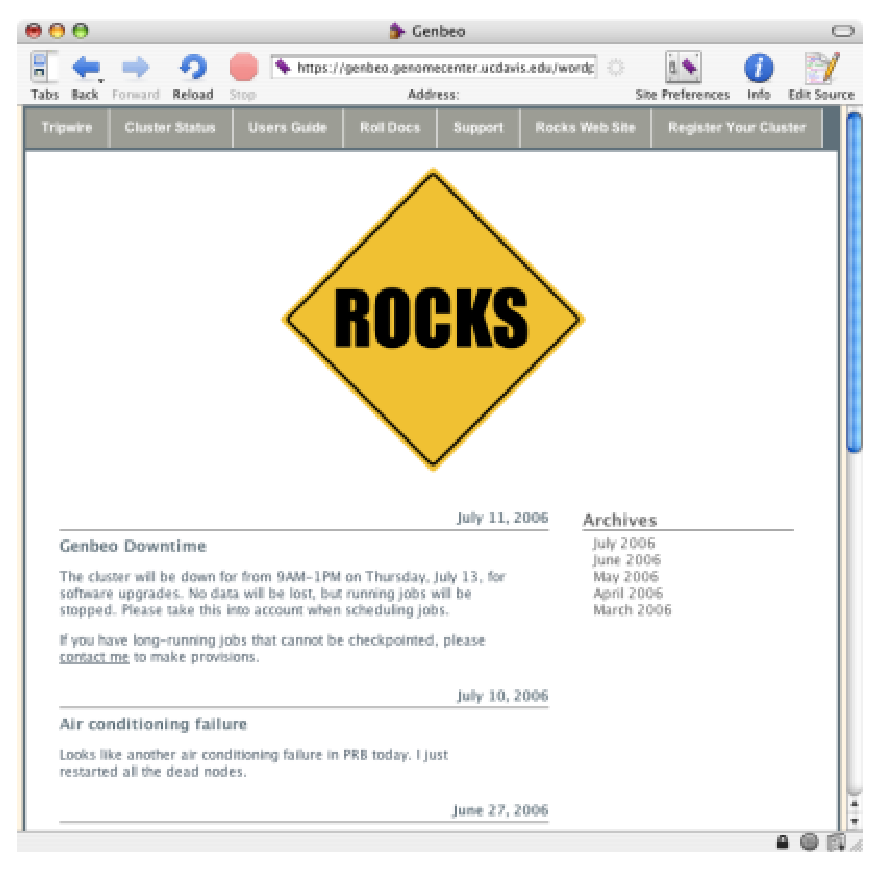
\includegraphics[height=6cm]{rocks-web-main.eps}
\end{center}
\end{slide}

\begin{slide}{Cluster Web Interface}
\begin{center}
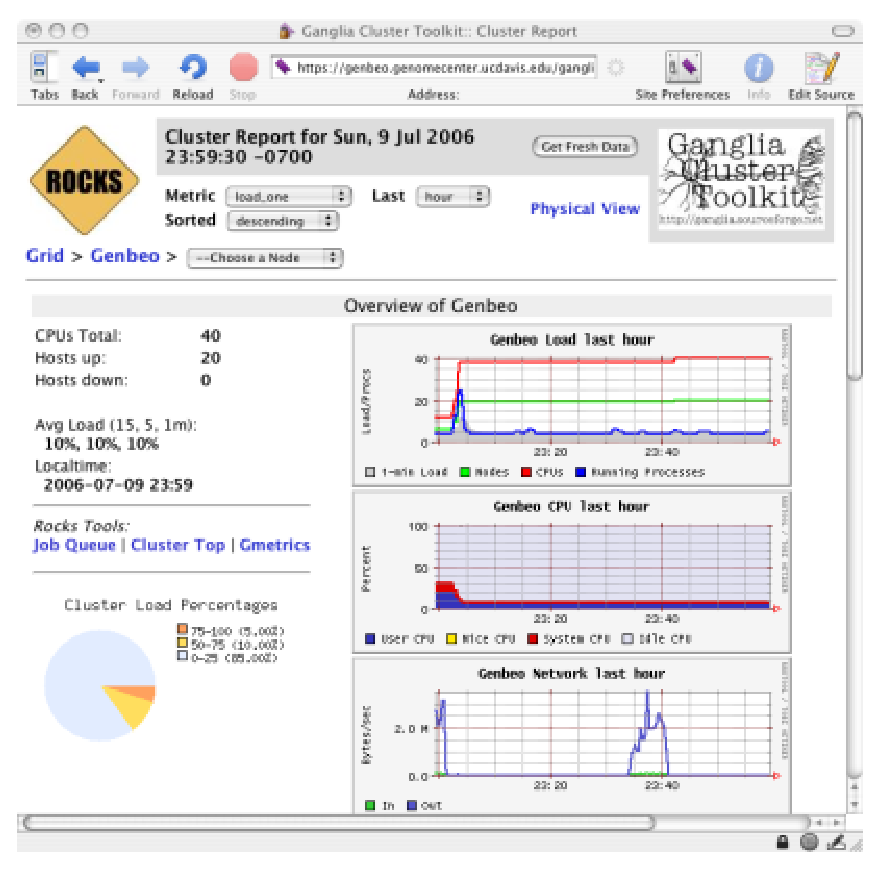
\includegraphics[height=6cm]{rocks-web-report.eps}
\end{center}
\end{slide}

\begin{slide}{Cluster Web Interface}
\begin{center}
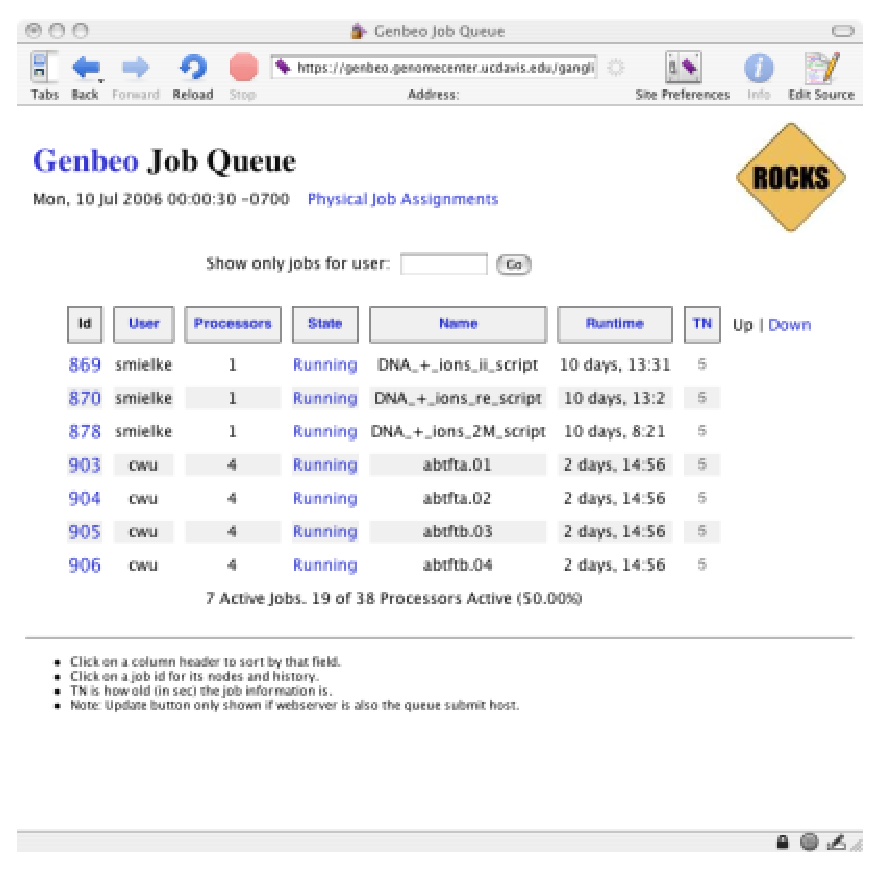
\includegraphics[height=6cm]{rocks-web-jobq.eps}
\end{center}
\end{slide}

\overlays{6}{%
\begin{slide}{Sun Grid Engine}
\begin{itemstep}
	\item What is a batch queue?
	\begin{itemize}
		\item Manage cluster resources
	\end{itemize}
	\item Why use the batch queue?
	\begin{itemize}
		\item Share cluster resources
		\item You don't need to worry about when/where your jobs run
		\item Submit a whole bunch of jobs and go home!
	\end{itemize}
\end{itemstep}
\end{slide}}

\overlays{3}{%
\begin{slide}{SGE Terminology: slots}
\begin{itemstep}
	\item A resource allocated to your job
	\item We define one slot per CPU core
	\item Can request number of slots when you submit job
\end{itemstep}
\end{slide}}

\overlays{5}{%
\begin{slide}{SGE Terminology: Parallel Environment}
\begin{itemstep}
	\item Need to use a PE when you want more than one slot
	\item PE can specify start and stop programs (eg mpirun)
	\item PEs avilable:
	\begin{itemize}
		\item serial
		\item mpich
	\end{itemize}
\end{itemstep}
\end{slide}}

\overlays{3}{%
\begin{slide}{SGE Terminology: Job Array}
\begin{itemstep}
	\item Run the same job multiple times
	\item submit/manage as a single job
	\item Ideal for running the same program repeatedly with different
         input files or parameters
\end{itemstep}
\end{slide}}

\overlays{9}{%
\begin{slide}{Queue example}
\begin{tabular}{ccc}
\begin{tabular}{|c|c|}
\hline
Job & Slots \\
\hline
\untilSlide{4}{\green $A$} 	& \untilSlide{4}{6} \\
\hline
\untilSlide{6}{\red $B_1$}		& \untilSlide{6}{1} \\
\untilSlide{7}{\red $B_2$}		& \untilSlide{7}{1} \\
\untilSlide{9}{\red $B_3$}		& \untilSlide{9}{1} \\
\hline
\untilSlide{9}{\blue $C$}		& \untilSlide{9}{4} \\
\hline
\end{tabular} 
&
\begin{tabular}{|c@{\hspace{.5cm}|c|}
\hline
\onlySlide*{2}{\green $A$}%
\onlySlide*{3}{\green $A$}%
\onlySlide*{4}{\green $A$}%
& 
\onlySlide*{2}{\green $A$}%
\onlySlide*{3}{\green $A$}%
\onlySlide*{4}{\green $A$}%
\\
\hline
\onlySlide*{2}{\green $A$}%
\onlySlide*{3}{\green $A$}%
\onlySlide*{4}{\green $A$}%
&
\onlySlide*{2}{\green $A$}%
\onlySlide*{3}{\green $A$}%
\onlySlide*{4}{\green $A$}%
\onlySlide*{6}{\red $B_3$}%
\onlySlide*{7}{\red $B_3$}%
\onlySlide*{8}{\red $B_3$}%
\onlySlide*{9}{\red $B_3$}%
\\
\hline
\end{tabular} 
&
\begin{tabular}{|c|c|}
\hline
\onlySlide*{2}{\green $A$}%
\onlySlide*{3}{\green $A$}%
\onlySlide*{4}{\green $A$}%
\onlySlide*{9}{\blue $C$}%
&
\onlySlide*{2}{\green $A$}%
\onlySlide*{3}{\green $A$}%
\onlySlide*{4}{\green $A$}%
\onlySlide*{9}{\blue $C$}%
\\
\hline
\onlySlide*{3}{\red $B_1$}%
\onlySlide*{4}{\red $B_1$}%
\onlySlide*{5}{\red $B_1$}%
\onlySlide*{6}{\red $B_1$}%
\onlySlide*{9}{\blue $C$}%
&
\onlySlide*{4}{\red $B_2$}%
\onlySlide*{5}{\red $B_2$}%
\onlySlide*{6}{\red $B_2$}%
\onlySlide*{7}{\red $B_2$}%
\onlySlide*{9}{\blue $C$}%
\\
\hline
\end{tabular}
\\
Queue & Node1 & Node2 \\
\end{tabular}
\vskip 0.75cm
\onlySlide*{1}{Three jobs waiting in queue...}%
\onlySlide*{2}{Job {\green $A$} is scheduled}%
\onlySlide*{3}{Job {\red $B_1$} is scheduled}%
\onlySlide*{4}{Job {\red $B_2$} is scheduled}%
\onlySlide*{5}{Job {\green $A$} finishes}%
\onlySlide*{6}{Job {\red $B_3$} is scheduled}%
\onlySlide*{7}{Job {\red $B_1$} finishes}%
\onlySlide*{8}{Job {\red $B_2$} finishes}%
\onlySlide*{9}{Job {\blue $C$} is scheduled}%
\end{slide}}

\overlays{4}{%
\begin{slide}{SGE Commands}
\begin{itemstep}
	\item qsub: submit jobs
	\item qstat: get job status
	\item qdel: remove a job
	\item qlogin: interactive login
\end{itemstep}
\end{slide}}

\begin{slide}{SGE Commands: qsub}
Use the {\tt qsub} command to submit a batch job to the system

Simplest case:
\tiny
\begin{verbatim}
$ qsub file.sh
Your job 929 ("file.sh") has been submitted.
\end{verbatim}
\end{slide}

\begin{slide}{SGE Commands: qstat}
\ptsize{12}
Use the {\tt -f} flag to see all jobs running...
\tiny
\begin{verbatim}
$ qstat -f
queuename                    qtype used/tot. load_avg arch        states
------------------------------------------------------------------------
all.q@compute-0-1.local      BIP   4/4       1.83     lx26-amd64
  2455 0.60500 proAwt     cwu         r     06/21/2006 12:06:06   4
------------------------------------------------------------------------
all.q@compute-0-10.local     BIP   0/4       0.00     lx26-amd64  d
------------------------------------------------------------------------
all.q@compute-0-98.local     BIP   4/4       2.80     lx26-amd64
  2823 0.51386 ccr5_SCH_A twang       r     07/07/2006 15:12:51   2
  2865 0.50500 rungb5b    xjdeng      r     07/08/2006 17:37:06   1
  2944 0.52905 g2l_ff03   zxwang      r     07/09/2006 22:07:21   1
------------------------------------------------------------------------
all.q@compute-0-99.local     BIP   0/4       0.00     lx26-amd64
\end{verbatim}
%\onlyslide*{1}{\rput[t](-0.5,1.25){
\includegraphics[width=.8cm]{arrow.eps}}}
%\onlyslide*{2}{\rput[t](-0.5,2.5){
\includegraphics[width=.8cm]{arrow.eps}}}
%\onlyslide*{3}{\rput[t](-0.5,3.25){
\includegraphics[width=.8cm]{arrow.eps}}}
%\onlyslide*{4}{\rput[t](-0.5,4){
\includegraphics[width=.8cm]{arrow.eps}}}
%\onlyslide*{5}{\rput[t](8.5,5.5){
\includegraphics[height=.8cm]{downarrow.eps}}}
%\onlyslide*{6}{\rput[t](7.5,5.5){
\includegraphics[height=.8cm]{downarrow.eps}}}
%\onlyslide*{7}{\rput[t](6,5.5){
\includegraphics[height=.8cm]{downarrow.eps}}}
%\onlyslide*{8}{\rput[t](5,5.5){
\includegraphics[height=.8cm]{downarrow.eps}}}
%\onlyslide*{9}{\rput[t](4,5.5){
\includegraphics[height=.8cm]{downarrow.eps}}}
%\onlyslide*{10}{\rput[t](1,5.5){
\includegraphics[height=.8cm]{downarrow.eps}}}
\end{slide}

\begin{slide}{SGE Commands: qstat}
\ptsize{12}
...as well as those waiting to be run.
\tiny
\begin{verbatim}
########################################################################
PENDING JOBS - PENDING JOBS - PENDING JOBS - PENDING JOBS - PENDING JOBS
########################################################################
2947 0.52905 g2f_ff03   zxwang       qw    07/09/2006 22:11:04    20
2948 0.52905 g2h_ff03   zxwang       qw    07/09/2006 22:11:55    20
2949 0.52905 g2q_ff03   zxwang       qw    07/09/2006 22:12:42    20
\end{verbatim}
\end{slide}

\begin{slide}{SGE Commands: qstat}
Use the {\tt -j <jobid>} flag to get more information about a job:
\tiny
\begin{verbatim}
$ qstat -j 2947
job_number:                 2947
exec_file:                  job_scripts/2947
submission_time:            Sun Jul  9 22:11:04 2006
...
\end{verbatim}
\end{slide}

\overlays{3}{%
\begin{slide}{SGE Commands: qdel}
\begin{itemstep}
\item Use the {\tt qdel} command to delete a previously scheduled job from the
queue.

\item Note: if the job was running, you may still have to kill the processes by
hand.

\item The {\tt -f} (force) option can sometimes be necessary to clean up jobs
left behind, for example, if a node dies during the job.
\end{itemstep}
\end{slide}}

\overlays{4}{%
\begin{slide}{SGE Commands: qlogin}
Use the {\tt qlogin} command to schedule an interactive login.
\begin{itemstep}
	\item Default is one slot
	\item To allocate more slots, use the parallel environment serial and the
         number of slots {\tt qlogin -pe serial 2}
	\item Two slots on genbeo will give you the whole node (4 on shiraz)
	\item If enough slots are not avilable, {\tt qlogin} will fail.
\end{itemstep}
\end{slide}}

\begin{slide}{SGE Example: BLAST}
\ptsize{12}
Single Threaded single app (simple) BLAST (Basic Local Alignment Search Tool)

SGE script: ({\tt sge\_blast.sh})
\tiny
\begin{verbatim}
# Blast executable binary
BLAST=/opt/Bio/blast-2.2.14/bin/blastall

#$ -cwd
#$ -o blastout
#$ -e blasterr
#$ -q all.q
#$ -S /bin/bash

$BLAST $*
\end{verbatim}
Lines with {\tt \#\$} are command-line flags for SGE.
\end{slide}

\overlays{5}{%
\begin{slide}{SGE Example: BLAST}
{\tiny \tt qsub -N serialBlast sge\_blast.sh -p blastp -i query.aa \\}
{\tiny \tt    -d drosoph.aa -e 1e-40 -o output.blast}
\begin{itemstep}
		\item {\tt -N} Specify job name ({\tt serialBlast})
		\item {\tt -q} Specify queue in which to run job ({\tt all.q})
		\item {\tt -S} Specify interpreter to run script ({\tt /bin/bash})
		\item {\tt -o} Specify file for stdout of job
		\item {\tt -cwd} Execute job in the directory from which it was submitted
\end{itemstep}
\end{slide}}

\begin{slide}{SGE Example: mpi-BLAST}
Parallel version of BLAST using MPI

SGE script: ({\tt sge\_mpiblast,sh})
\tiny
\begin{verbatim}
# Basic SGE script to run mpiblast

MPIRUN=/opt/mpich/gnu/bin/mpirun
MPIBLAST=/opt/Bio/mpiblast-1.4.0/bin/mpiblast

#$ -cwd
#$ -o mpiblastout
#$ -e mpiblasterr
#$ -q all.q
#$ -S /bin/bash

$MPIRUN -np $NSLOTS -machinefile /$TMPDIR/machines $MPIBLAST $*
\end{verbatim}
\end{slide}

\begin{slide}{SGE Example: mpi-BLAST}
{\tiny \tt qsub -N mpiblast1 -pe mpich 4 sge\_mpiblast.sh -p blastp \\}
{\tiny \tt    -d swissprot -i query.aa -o mpiblast.out -e 1e-40}
\begin{itemstep}
	\item {\tt -pe} Specify parallel environment and number of slots
\end{itemstep}
\end{slide}

\overlays{2}{%
\begin{slide}{SGE Example: R}
\begin{itemstep}
	\item {\tt -t 1-5:1}
	\item {\tt -hold\_jid job-name-or-id}
\end{itemstep}
\end{slide}}

\begin{slide}{SGE Example: qlogin}
\end{slide}

\overlays{3}{%
\begin{slide}{Things to do}
\begin{itemstep}
	\item Use the scheduler!
	\item Checkpoint your job
	\item Make use of local storage on the nodes for intermediate results
\end{itemstep}
\end{slide}}

\overlays{3}{%
\begin{slide}{Things NOT to do}
\begin{itemstep}
	\item Run jobs on the head node
	\item Many simultaneous writes to network filesystem
	\item Go around scheduler and run directly on the nodes
\end{itemstep}
\end{slide}}

\begin{slide}{The end}
\begin{itemstep}
	\item Get an account: 
		{\tiny \tt http://genomecenter.ucdavis.edu/}, click on "Administration"

	\item Documentation and example scripts: 
		{\tiny \tt http://wiki.genomecenter.ucdavis.edu/bioinformatics/}

	\item Questions?
\end{itemstep}
\end{slide}

\end{document}
